\documentclass[11pt,a4paper]{article}

\usepackage[margin=2.5cm]{geometry}
\usepackage[T1]{fontenc}
\usepackage{lmodern}
\usepackage{microtype}
\usepackage{graphicx}
\usepackage{booktabs}
\usepackage{amsmath}
\usepackage{siunitx}
\usepackage{caption}
\usepackage[hidelinks]{hyperref}
\usepackage[numbers,sort&compress]{natbib}

\captionsetup{font=small,labelfont=bf}
\sisetup{group-separator={,},group-minimum-digits=4,group-digits=integer}

\title{From Raw Micro-CT Slices to Individual Tooth Models:\\
Open Tools for Shimadzu inspeXio Data in 3D~Slicer}
\author{Nobuhiko Hata, PhD\\[2pt]
\small Surgical Robotics and Navigation Laboratory, Department of Radiology\\
\small Brigham and Women's Hospital and Harvard Medical School, Boston, MA, USA\\
\small \texttt{hata@bwh.harvard.edu}}
\date{White paper, November 2026}

\begin{document}
\maketitle

\begin{abstract}
Laboratory micro-CT scanners write their reconstructions in vendor formats that general-purpose medical imaging software does not read, and the grey values they produce are not calibrated to Hounsfield units, so even viewing a scan in 3D~Slicer can require reverse engineering. This white paper describes an open workflow that takes a Shimadzu inspeXio reconstruction from its raw slice files to individually segmented tooth models. We show that the inspeXio \texttt{.cb} slice files are uncompressed 16-bit TIFF images, so that a detached NRRD header is enough to load a reconstruction in 3D~Slicer without copying any pixel data, and we derive volume rendering settings from the measured grey values of the specimen. We then report on segmentation. In the specimen studied, the teeth are embedded in a base material of almost the same density as dentin. Thresholding therefore recovered only the crowns, and a deep-learning model trained on clinical cone-beam CT labelled the base material as tooth. The promptable foundation model nnInteractive, given one two-dimensional box per tooth and a few corrective points for two teeth, segmented nine teeth with their roots in about four seconds per tooth on a consumer GPU. The converter, the scripts and step-by-step guides are released in two public repositories.
\end{abstract}

\section{Introduction}

Micro-CT is widely used to study the morphology of teeth and bone because it resolves structures of a few tens of micrometres in three dimensions. Turning a micro-CT scan into quantitative anatomy, however, usually means moving the data from the scanner's own software into a general analysis environment, and this step is often harder than it should be. Vendor reconstruction formats are rarely documented, the grey values are scanner units rather than calibrated densities, and published segmentation tools for dental anatomy are trained on clinical cone-beam CT (CBCT), whose resolution, noise and contrast differ substantially from those of a laboratory scan of an embedded specimen.

3D~Slicer~\cite{fedorov2012slicer} is a natural destination for such data, since it combines visualization, segmentation and an embedded Python environment in a free and open platform. This white paper describes how a Shimadzu inspeXio micro-CT reconstruction of a dental specimen was brought into 3D~Slicer and segmented into individual teeth, and it reports the approaches that did not work as well as the one that did, because the failures explain the final design. The resulting tools are a format converter with a volume rendering guide~\cite{repoConverter} and a tooth segmentation package~\cite{repoSegmentation}.

\section{Data}

The example scan, \texttt{lot261019\_M1\_Fgfr3++\_no\_gel\_dpi1w2\_cb\_000}, was acquired on a Shimadzu inspeXio scanner in cone-beam mode at \SI{100}{\kilo\volt} and \SI{200}{\micro\ampere}, with a source-to-detector distance of \SI{500}{\milli\metre} and a source-to-rotation-axis distance of \SI{350}{\milli\metre}, according to the acquisition screenshot stored with the data. The reconstruction consists of 880 slices of $1024 \times 1024$ voxels with a field of view of \SI{45.5}{\milli\metre} in plane and \SI{39.1}{\milli\metre} along the rotation axis. The scanner also wrote a second reconstruction of the same acquisition into a subfolder named \texttt{noring\_0000}.

\section{Reading the inspeXio format}

Each reconstruction folder holds one \texttt{.cb} file per slice together with per-slice \texttt{.inf} and \texttt{.prm} files and a text file that states the pixel size. Inspection of the bytes showed that every \texttt{.cb} file is an uncompressed, little-endian, 16-bit TIFF image whose pixel data occupy one contiguous block that starts after a 1,372-byte header. The pixel size, \SI{0.0443945}{\milli\metre}, is given in \texttt{0000.txt}, and the acquisition screenshot reports the same voxel size along the rotation axis, which is also what the axial field of view divided by the number of slices gives, so the voxels are isotropic.

Because all slices share the same size and header length, a detached NRRD header that lists the 880 slice files and instructs the reader to skip the first 1,372 bytes of each is sufficient for 3D~Slicer to load the full volume. No pixel data are copied, so the header is a few kilobytes for a 1.8~GB volume. The converter \texttt{cb2nrrd.py}~\cite{repoConverter} generalizes this observation. It reads the image size, bit depth, byte order and data offset from the TIFF tags of each file and the voxel size from the text file, it checks that all slices share one layout and that the slice numbering has no gaps, and it then writes either the detached header or a self-contained, optionally compressed NRRD file. The converter needs only the Python standard library for headers and NumPy for full files, and it runs inside 3D~Slicer's Python console as well. A comparison of the two reconstructions on the middle slice (Fig.~\ref{fig:ring}) showed that \texttt{noring\_0000} is the ring-artifact-corrected version, so it was used throughout.

\begin{figure}[t]
\centering
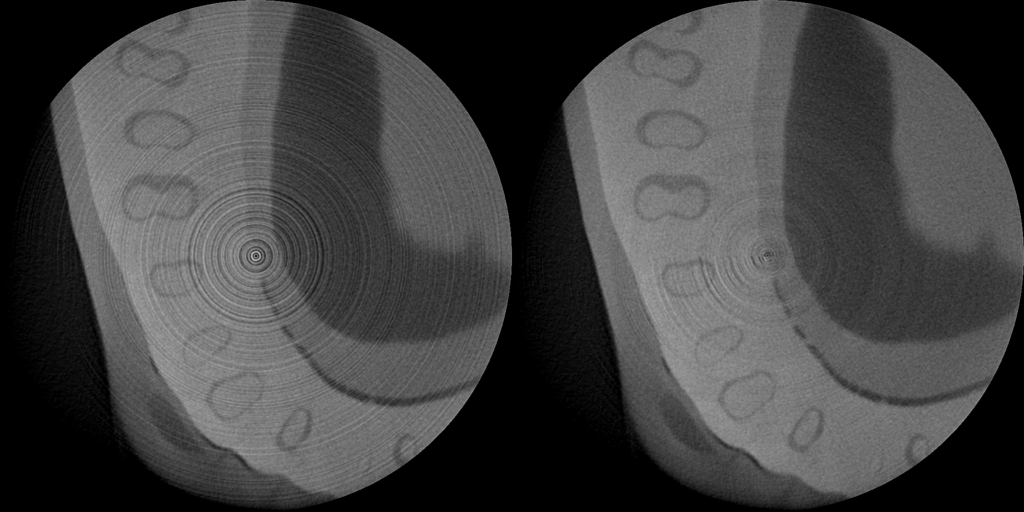
\includegraphics[width=0.8\linewidth]{../docs/images/history_ring_artifact.png}
\caption{Middle slice of the original reconstruction (left) and of the ring-corrected reconstruction in \texttt{noring\_0000} (right).}
\label{fig:ring}
\end{figure}

\section{Volume rendering}

Since the grey values are scanner units, the computed-tomography presets of 3D~Slicer did not apply, and the first renderings illustrated how sensitive the result is to the opacity transfer function. A cutoff of 37,500 made the whole cylindrical field of view opaque, whereas a cutoff of 38,800 rendered the teeth as fragments. Measurement of a slice through the teeth resolved the question. The background and holder lie near 34,700, the soft material around the teeth near 37,200, and the teeth and bone between about 38,100 and 39,800, so an opacity ramp from 37,800 to 39,000 shows complete teeth while keeping the surrounding material transparent. Because bone of the same density covers the teeth when they are seen from above, the camera was turned to view the arch from the occlusal side (Fig.~\ref{fig:vr}). These settings are reproduced by a single script, \texttt{render\_in\_slicer.py}, which also prints a grey-value histogram so that the thresholds can be set for other scans~\cite{repoConverter}.

\begin{figure}[t]
\centering
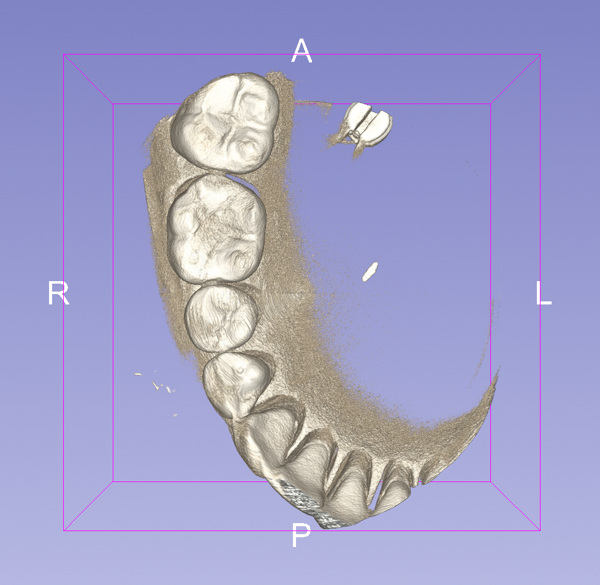
\includegraphics[width=0.48\linewidth]{../docs/images/history_volume_rendering.png}
\caption{Volume rendering of the teeth viewed from the occlusal side, with opacity rising from grey value 37,800 to 39,000.}
\label{fig:vr}
\end{figure}

\section{Segmentation approaches that fell short}

\subsection{Thresholding}

Enamel is the brightest material in the specimen, so a threshold at about 38,800 after Gaussian smoothing, followed by a morphological opening that removes the thin wall of the sample tube and a slice range that excludes the holder, isolated the crowns well on a reduced copy of the scan. At full resolution, however, the same procedure produced a large cylindrical shell (Fig.~\ref{fig:fail}, left), which revealed a thin bright rim at the edge of the circular reconstruction field of view. The rim can be masked, but thresholding faced a more fundamental limit. The roots are embedded in a base material whose grey value is nearly that of dentin, and the only boundary between them is a thin dark outline, so no global threshold separates roots from base.

\subsection{A CBCT-trained dental model}

The CBCTToothSegmentation extension for 3D~Slicer~\cite{kitwareCBCT} runs a three-dimensional U-Net, implemented with MONAI~\cite{cardoso2022monai}, inside a region of interest drawn around each tooth. Running it on Slicer~5.12 required replacing the pinned MONAI version~1.3.0, which does not import under Python~3.12, with a current release. Because the model normalizes intensities within the region of interest but does not resample, and because it pads each region to 144 voxels by mirroring, the scan also had to be resampled to coarser, CBCT-like voxels. At \SI{0.15}{\milli\metre} and \SI{0.3}{\milli\metre}, with and without flattening the base to background intensity, the model either filled its regions with base material (Fig.~\ref{fig:fail}, right) or returned small fragments. We attribute this to the contrast on which such models rely, since a tooth in clinical CBCT is much brighter than the surrounding soft tissue, whereas here tooth and base have nearly the same grey value.

For the same reason two further options were not pursued. The fully automatic system of Cui et~al.~\cite{cui2022fully} segments individual teeth and alveolar bone with high accuracy on clinical CBCT, but its trained weights are not publicly released. DentalSegmentator~\cite{dot2024dentalsegmentator}, an nnU-Net~\cite{isensee2021nnunet} model available in 3D~Slicer, is likewise trained on CT and CBCT, and it labels the upper and lower teeth as two segments rather than as individual teeth.

\begin{figure}[t]
\centering
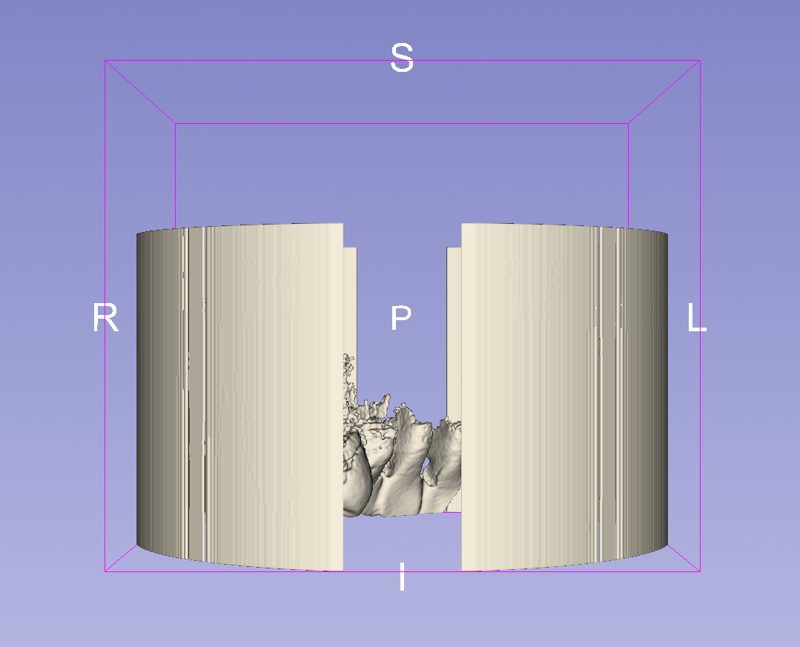
\includegraphics[height=5.2cm]{../docs/images/history_threshold_rim_shell.png}\hfill
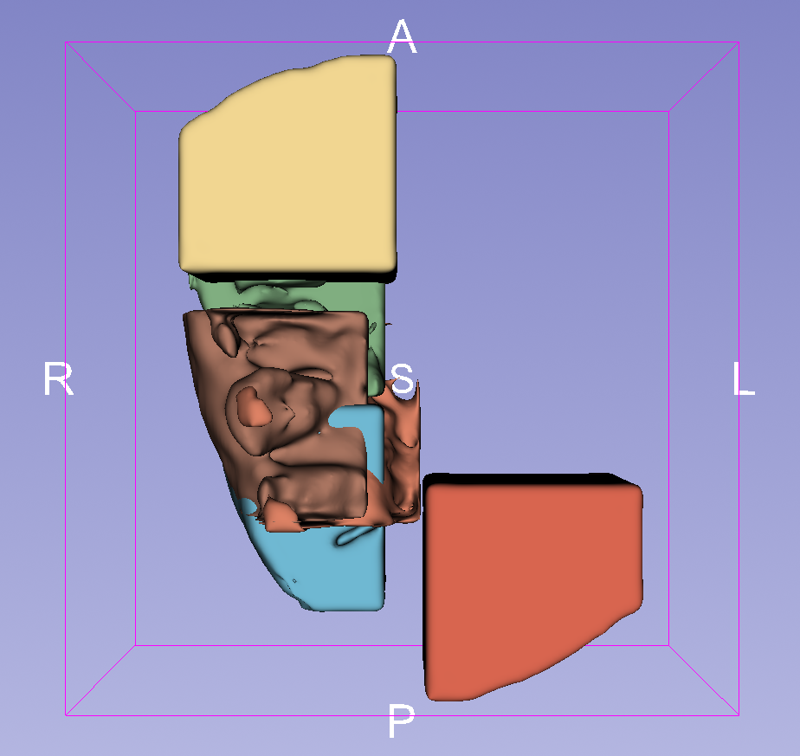
\includegraphics[height=5.2cm]{../docs/images/history_cbct_model_boxes.png}
\caption{Two failure modes. Left: thresholding at full resolution picks up a bright rim at the edge of the reconstruction field of view. Right: a CBCT-trained tooth model fills its regions of interest with base material.}
\label{fig:fail}
\end{figure}

\section{Promptable segmentation with nnInteractive}

\subsection{Method}

nnInteractive~\cite{isensee2025nninteractive} is a promptable three-dimensional segmentation model trained on more than 120 volumetric datasets spanning CT, MRI, PET and 3D microscopy, and it segments the object indicated by points, scribbles, lassos or boxes. Its 3D~Slicer integration~\cite{devente2026slicernninteractive} was not available in the Extensions Manager for Slicer~5.12.4, so the nnInteractive Python package (version~2.6.0, model checkpoint v1.0) was installed into Slicer's Python environment and driven by a script~\cite{repoSegmentation}. The script averages $2\times2\times2$ voxels of the slices that contain the teeth, which gives \SI{0.089}{\milli\metre} voxels, reduces noise and keeps the volume small enough for a GPU with \SI{12}{\giga\byte} of memory. For each tooth it then applies one prompt, adds optional negative or positive points, keeps the largest connected component, stores the result as a separate segment and exports a surface model.

Each prompt is a two-dimensional box on a vertical plane through the middle of the tooth, spanning the width of the crown, including both roots of a molar, and extending from the crown tip to just beyond the root apex (Fig.~\ref{fig:prompts}). Initial boxes were derived automatically from a map of the enamel crowns seen from the occlusal side, in which a distance-transform watershed separated touching crowns and the parts of each multi-cusped crown were merged by hand into one tooth.

\begin{figure}[t]
\centering
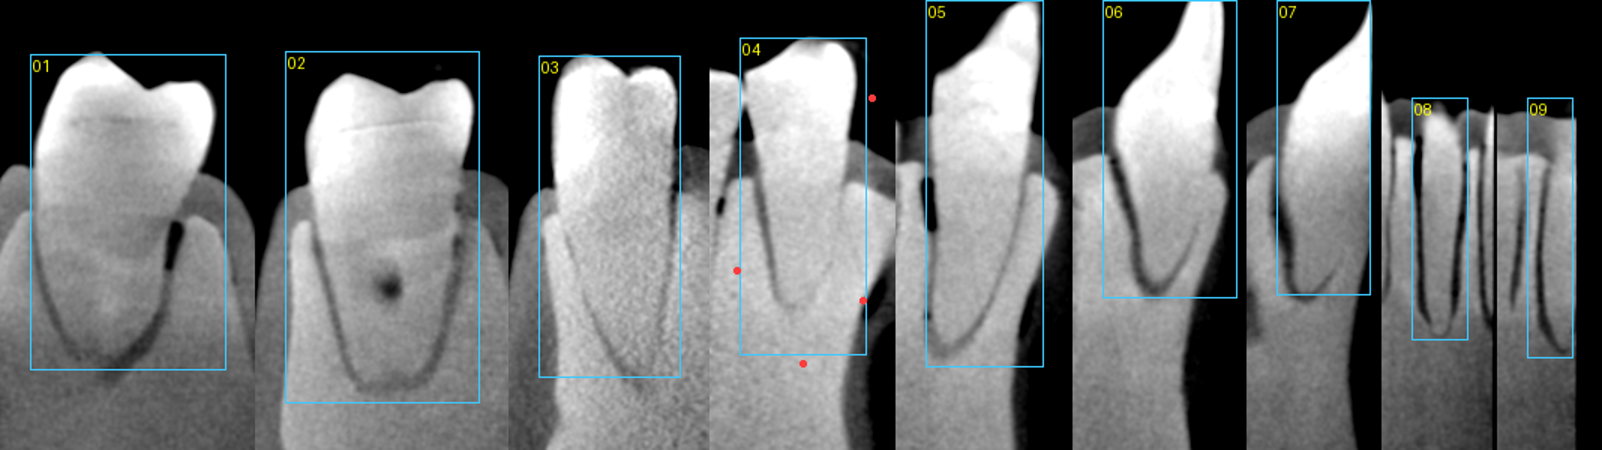
\includegraphics[width=\linewidth]{../docs/images/prompt_planes.png}
\caption{Prompt boxes (blue) on the vertical plane through each tooth, from crown tip to just beyond the root apex. Red dots mark negative points that lie on the plane shown.}
\label{fig:prompts}
\end{figure}

\subsection{Lessons from refining the prompts}

Three observations shaped the final prompts. First, the length of the box matters, because nnInteractive treats the box as the extent of the object. A rule that lengthened any box whose segmentation reached its lower edge made the two large molars grow into the base to more than \SI{2000}{\cubic\milli\metre} each, so every box was instead set to end just beyond the root apex as read from the dark outline in the slices. Second, two teeth still leaked into the base, and four and seven negative points placed in the leaked regions corrected them. Third, two front teeth were missed by the crown map because their crowns lie beyond the top of the scanned volume, and their boxes were added by hand on the planes of their roots.

\subsection{Results}

The final prompts produced nine separate teeth, each with crown and roots (Fig.~\ref{fig:result}). Each tooth outline followed the dark line around its root on the plane of its prompt (Fig.~\ref{fig:outlines}). After the model had been loaded, which took about a minute on first use including the download of the weights, each tooth required 3--5~s on an NVIDIA GeForce RTX~3060 with \SI{12}{\giga\byte}. Table~\ref{tab:volumes} lists the prompts and the resulting volumes. The volumes of teeth 05--09 are incomplete because their crowns extend beyond the scanned volume, and these teeth therefore end flat at the top.

\begin{figure}[t]
\centering
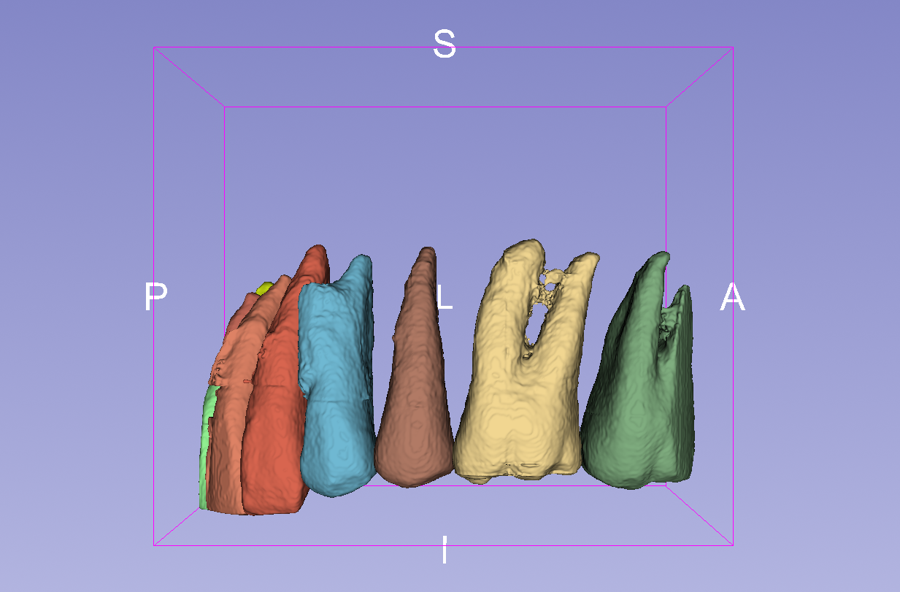
\includegraphics[height=5.6cm]{../docs/images/nnInteractive_teeth_side.png}\hfill
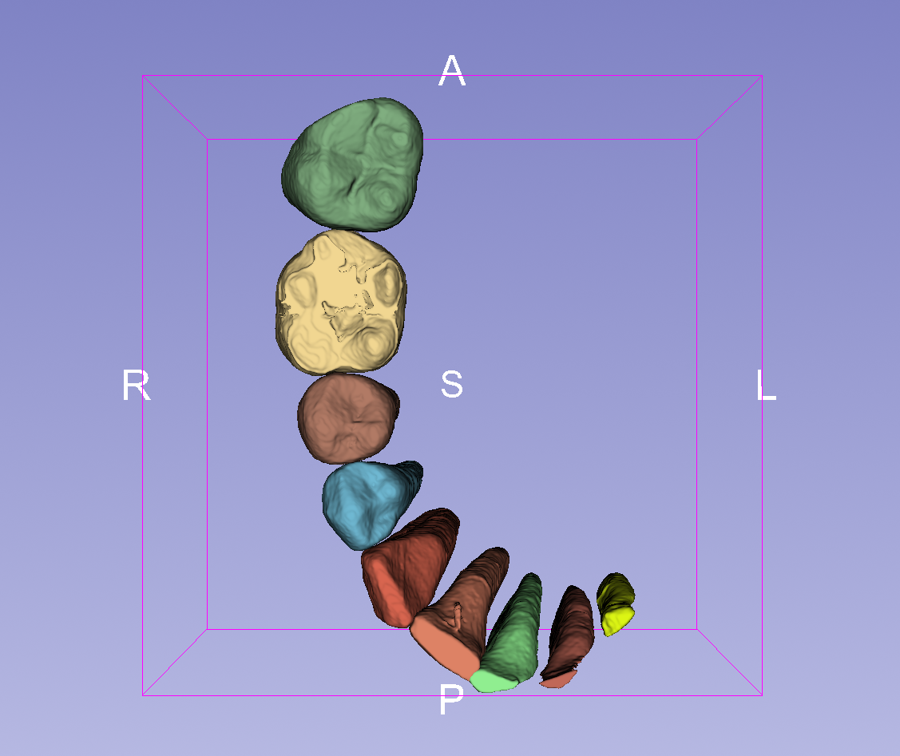
\includegraphics[height=5.6cm]{../docs/images/nnInteractive_teeth_occlusal.png}
\caption{Nine teeth segmented with nnInteractive, shown as surface models from the side (left, crowns at the bottom) and from the occlusal side (right).}
\label{fig:result}
\end{figure}

\begin{figure}[t]
\centering
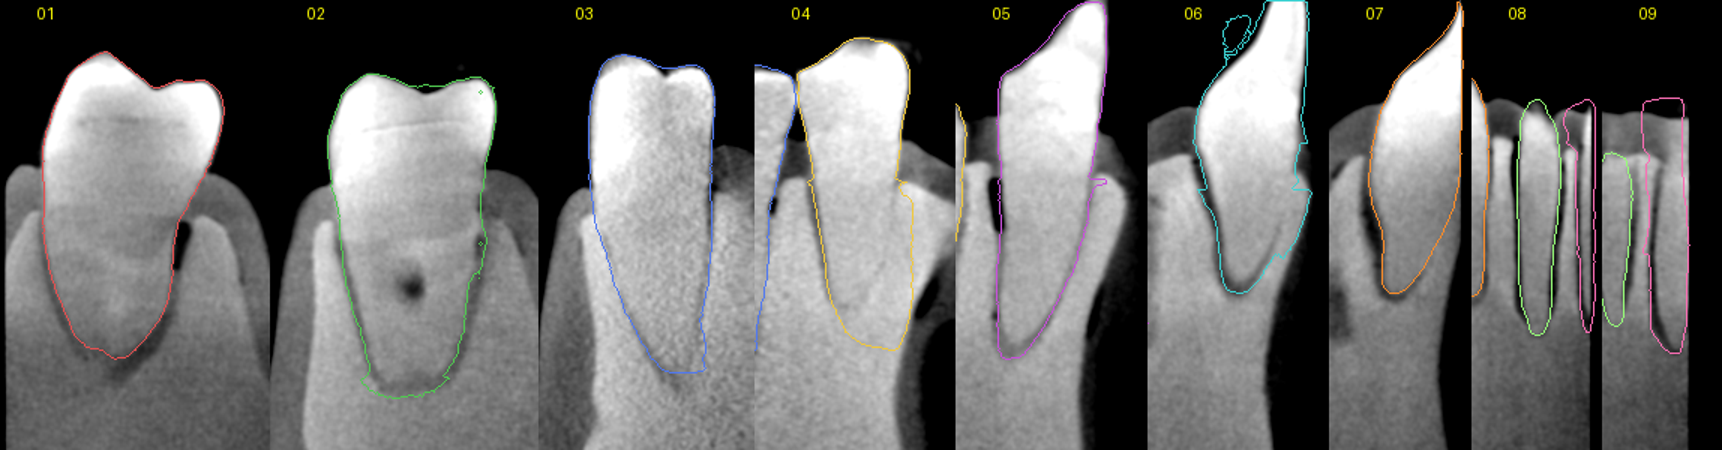
\includegraphics[width=\linewidth]{../docs/images/nnInteractive_outlines.png}
\caption{Outline of each segmented tooth on the plane of its prompt.}
\label{fig:outlines}
\end{figure}

\begin{table}[t]
\centering
\caption{Prompts and segmented volumes at \SI{0.089}{\milli\metre} voxel size. Volumes of teeth 05--09 are incomplete because their crowns lie outside the scanned volume.}
\label{tab:volumes}
\begin{tabular}{llr}
\toprule
Tooth & Prompt & Volume (\si{\cubic\milli\metre}) \\
\midrule
01 & box & 887 \\
02 & box and 4 negative points & 1160 \\
03 & box & 466 \\
04 & box and 7 negative points & 451 \\
05 & box & 473 \\
06 & box & 371 \\
07 & box & 219 \\
08 & box & 117 \\
09 & box & 66 \\
\bottomrule
\end{tabular}
\end{table}

\section{Discussion}

Most of the progress in this work came from examining the data closely rather than from any single tool. The undocumented slice format proved to be ordinary TIFF once its bytes were read, the volume rendering became meaningful only after the grey values of the specimen had been measured, and the bright rim at the edge of the field of view appeared only at full resolution. The failures were equally informative. Because the roots and the embedding base have nearly the same density, neither a threshold nor a model that expects the contrast of clinical CBCT could separate them, whereas a general promptable model succeeded because it follows the boundary that the prompt points to. Even so, the prompts had to be fitted to the anatomy, box by box, which suggests that interactive rather than fully automatic segmentation is the realistic choice for specimens that differ from the data a model was trained on.

The work has limitations. The method was demonstrated on a single scan, and the segmentations were checked visually against the root outlines rather than against a manual reference segmentation, so accuracy was not quantified. The prompts were partly derived by hand, the downsampling to \SI{0.089}{\milli\metre} trades fine detail for memory, and the crowns of the front teeth were outside the scanned volume. The nnInteractive weights are licensed for non-commercial use only (CC~BY-NC-SA~4.0). Natural next steps are a comparison with manual segmentation on several specimens, automatic proposal of prompts from the crown map inside 3D~Slicer, and interactive prompting once the nnInteractive extension is available for current Slicer releases.

\section{Availability}

The converter and the volume rendering guide are available at \url{https://github.com/nobyhata/Shimadzu-inspeXio-converter-for-3D-Slicer}~\cite{repoConverter}. The segmentation script, the prompts for the example scan, a step-by-step guide and a narrative history of the work are available at \url{https://github.com/nobyhata/inspeXio-3D-Teeth-Segmentation}~\cite{repoSegmentation}. The workflow was tested with 3D~Slicer~5.12.4 on Windows.

\section*{Acknowledgments}

The data analysis, scripting and drafting of this white paper were carried out with the assistance of Claude (Anthropic), an AI assistant, under the direction of the author, who reviewed the results.

\bibliographystyle{unsrtnat}
\bibliography{references}

\end{document}
